\documentclass[a4paper,11pt]{article}
\usepackage[utf8]{inputenc}
\usepackage{listings}
\usepackage{mathtools}   % need for subequations
\usepackage{graphicx}   % need for figures
\usepackage{verbatim}   % useful for program listings
\usepackage{color}      % use if color is used in text 
\usepackage{url}
\usepackage{todonotes}
\usepackage{tikz}
\usetikzlibrary{arrows}
\usepackage{enumitem}
\usepackage{pdfpages}
\usepackage{subcaption}
\usepackage{amsfonts}
\usepackage{latexsym}
\usepackage[T1]{fontenc} % use for allowing < and > in cleartext
\usepackage{fixltx2e}    % use for textsubscript
\usepackage[titletoc,title]{appendix}
\usepackage[framemethod=tikz]{mdframed}
\usepackage[titletoc,title]{appendix}

\usepackage[margin=2.5cm]{geometry}
\usepackage[ampersand]{easylist}
\usepackage{epstopdf}
\usepackage{algorithm}
\usepackage{algpseudocode}
\renewcommand{\algorithmicforall}{\textbf{for each}}
\makeatletter
\def\BState{\State\hskip-\ALG@thistlm}
\makeatother
\usepackage{float}
\usepackage[hypcap=false]{caption}
\usepackage{hyperref}
\DeclareCaptionFormat{algor}{%
  \hrulefill\par\offinterlineskip\vskip1pt%
    \textbf{#1#2}#3\offinterlineskip\hrulefill}
\DeclareCaptionStyle{algori}{singlelinecheck=off,format=algor,labelsep=space}
\captionsetup[algorithm]{style=algori}

\definecolor{codegreen}{rgb}{0,0.6,0}
\definecolor{codegray}{rgb}{0.5,0.5,0.5}
\definecolor{codepurple}{rgb}{0.58,0,0.82}
\definecolor{backcolour}{rgb}{1.0,1.0,1.0}
\lstdefinestyle{mystyle}{
  backgroundcolor=\color{backcolour},   commentstyle=\color{codegreen},
  keywordstyle=\color{magenta},
  numberstyle=\tiny\color{codegray},
  stringstyle=\color{codepurple},
  basicstyle=\footnotesize,
  breakatwhitespace=false,         
  breaklines=true,                 
  captionpos=b,                    
  keepspaces=true,                 
  numbers=left,                    
  numbersep=5pt,                  
  showspaces=false,                
  showstringspaces=false,
  showtabs=false,                  
  tabsize=2
}
\lstset{style=mystyle}


\bibliographystyle{plain}

\begin{document}

\setlength{\parindent}{0cm}
\setlength{\unitlength}{1mm}
\date{December 17th 2014\\ IT University of Copenhagen}
\title{Actors In Movies\\SAD2 Fall 2014}

\author{Sarah de Voss\\
\texttt{satv@itu.dk}
\and Elvis Flesborg\\
\texttt{efle@itu.dk}
\and Mads Westi\\
\texttt{mwek@itu.dk}}
\clearpage\maketitle

\thispagestyle{empty}
\newpage
\tableofcontents
\thispagestyle{empty}
\newpage

\setcounter{page}{1}
\section{Finding a Similar Actor}

Say you want to make a movie with a specific actor in the leading role, but the actor is unavailable. You have already written the script, and found all the other actors. The only thing missing is the lead actor. \\

You find a similar actor. You find the most similar actor. And for this we must assume that, what defines an actor, is what movies it appears in. So you find the actor that has the most movies in common with your intended actor, and use that actor instead. \\

The size of a database expands every day with new entries. The IMDB (Intenet Movie Database) contains at this moment 817718 actors and 388215 movies. Checking for comparisons is labourous work even for a pc. The amount of comparisons is $O(a^2\cdot m)$ where $n$ is the number of actors and $m$ is the number of movies. This gives us $2.6\cdot 10^{17}$ comparisons!\\

For solving this problem we have created an algorithm that does similarity search through the \emph{IMDB database} and implemented different approximation schemes and compressed data to make the process faster without loosing too much accuracy.


\section{Implementation}
%\begin{mdframed}[hidealllines=true,backgroundcolor=blue!20]
We would like to find a similar actor to replace our unavailable lead actor. When is an actor similar to another? We start by discussing similarity and which similarity measure we are using. We then discuss measuring running time.\\
%\end{mdframed}

We are using Python to implement our algorithms as this is our language of choice. \\

We will look at the naïve solution, then \emph{MinHashing}, and then \emph{Locality Sensitive Hashing}, this is part one of the report. After that we will implement \emph{b-bit}, which is the extension to our report.\\

For each algorithm we will explain how it works and then go on to explain how we implemented it. We then explain the time and space complexity and the tradeoffs in accuracy. We finish each section with a discussion.\\


\subsection{Measuring similarity}
An actor has starred in a series of movies. This set\footnote{To compare sets of documents, the normal procedure is to convert them into shingles. But since the "documents" we are working on, are actual sets of index numbers, there is no need for us to use shingles} of movies we will call $S_1$. Another actor has starred in another set of movies $S_2$. We can measure the similarity between these actors using the Jaccard similarity index. It takes the intersection of the 2 sets and divides it by the union of the 2 sets. The Jaccard index falls in the range of 0-1. It is 1 if the sets are identical, and it is 0 if the sets are disjoint.

\begin{equation}
\text{Jaccard similarity index} (S_1, S_2) = \frac{|S_1 \cap S_2|}{|S_1 \cup S_2|}
\end{equation}



\subsection{Measuring Running Time}
\todo{And are we doing this at all?}

For every new implementation, we will measure the actual running time. It will be measured on a normal laptop computer with 8GB RAM and and intel i5 quadcore. If the running time takes longer than our patience permits, we will just put in how long we waited, and note that we did not run it through.\\

We will also create some random dummy data to run. This way we will be able to graph the running times, and look at the tendency curves. In the dummy data, there are 10 times as many actors, as there are movies. This corresponds pretty well with the \emph{imdb-r.txt} file, which has 63,594 distinct movies, and 460,428 distinct actors (not counting the movies with nonexisting movie-ids, and also not counting the movies with a ranking of \emph{NULL}).\\

But even though there are 10 more actors per movies many of these actors are only in one movie, and only few actors are in many movies. If we calculate the average number of movies, that an actor appears in, it is about 3. This will be taken into account when creating the dummy data. \\

One could argue that we could use a minimum rank as a cutoff on the original dataset, to simulate dummy data. But when we generate it randomly ourselves, we have (almost) full control over how many objects are created. \\


\subsection{Naïve Implementation}
Our starting point is to implement the naive solution, which has time complexity $O(n^2m)$, which is impossible to run on a normal laptop computer within the time span of this project. The correctness of this solution will be $100\%$.\\

\subsubsection{Data representation}
An actor is represented as a set of movies\footnote{Corresponding to the ids of the movies, which are integers} the specific actor appear in.

\begin{equation}
a_1 = \{m_1, m_2, m_3, \ldots , m_i\}
\end{equation}

Instead of storing the actors as sets, for reasons that become more apparent in section \ref{sec:minhashing}, it is beneficial to view the data as a binary characteristic matrix, where the rows are movies, the columns are actors and the values of the matrix defines whether an actor starred in a given movie or not.\\ 

\begin{figure}[!htbp]
\begin{eqnarray*}
 & a \ \text{actors} \\
 m \ \text{movies} = & 
\begin{cases}
    \overbrace{
    \begin{bmatrix}
        1 & 0 & 1 & 0 & 0 & 0 & 1\\
        1 & 0 & 0 & 1 & 0 & 0 & 1\\
        0 & 1 & 0 & 1 & 0 & 1 & 0\\
        0 & 1 & 0 & 1 & 0 & 0 & 0\\
        0 & 1 & 0 & 1 & 0 & 0 & 1\\
        1 & 0 & 1 & 0 & 0 & 0 & 1\\
        1 & 0 & 1 & 0 & 1 & 0 & 0
    \end{bmatrix} 
    }
\end{cases}
\end{eqnarray*}
\caption{Example of a characteristic matrix}
\label{fig:char_matrix}
\end{figure}

If we were to save the data as the full matrix as seen in ~\ref{fig:char_matrix}, the space complexity would be $\Theta (n \cdot m)$. In the actual implementation, \todo{reference til koden} the characteristic matrix is stored as a dictionary with a tuple $(a_i,m_j)$ as key, corresponding to an actor $i$ appearing in a movie $j$. This gives us constant lookup time and avoids storing 0's in the matrix\footnote{As suggested in \cite{book:mmds} p. 81}. The space complexity is still upper bound by $(n \cdot m)$, but since the matrix in most cases is very sparse, the average space consumption is much less. In our case with the IMDB data set where $s$ is the number of ones:
\begin{equation}
\begin{aligned}
a &= 460428\\
m &= 63594\\
s &= 1323388\\
ratio &= \frac{1323388}{63594 \cdot 460428} = 4.52\cdot 10^{-5}
\end{aligned}
\end{equation}

The naïve solution \todo{reference til koden} is calculating the Jaccard similarity using the characteristic matrix dictionary $D$, by looping through all pairs of actors, and for each pair loop through all the movies. We define $x = |S_1 \cap S_2|$\footnote{i.e the number of movies for which $D$ contains an entry for booth actors}. If we view the set union as $|S_1 \cup S_2| = |S_1 \oplus S_2| + |S_1 \cap S_2|$, we can define $y = |S_1 \oplus S_2|$\footnote{i.e the symmetric difference of the sets, the number of movies for which there are an entry for either one actor or the other in $D$}. The Jaccard similarity can therefore be computed as:

\begin{equation}
J(S_1,S_2) = \frac{x}{x+y}
\end{equation}

Because we have to construct every possible pair of actors and for each pair check if they appear in all movies, resulting in three nested for loops, the time complexity is $O(n^2 \cdot m)$, where $n$ is the number of distinct actors, and $m$ is the number of movies. Since this will not fit in memory on an average computer, a more sophisticated solution is needed. \\

\subsubsection{Actual Running Time}
The actual running time with the naïve implementation takes too long for our normal laptop computer and outruns our patience. We ran the implementation on random dummy datasets, which can be seen in figure ~\ref{fig:naive_at}. This figure is not very exciting in itself, but when we plot it together with the actual running times for the other implementations like MinHashing and Locality Sensitive Hashing, it will show how bad the naive implementation is. \\

\begin{figure}[!htbp]
    \begin{center}
        % GNUPLOT: LaTeX picture with Postscript
\begingroup
  \makeatletter
  \providecommand\color[2][]{%
    \GenericError{(gnuplot) \space\space\space\@spaces}{%
      Package color not loaded in conjunction with
      terminal option `colourtext'%
    }{See the gnuplot documentation for explanation.%
    }{Either use 'blacktext' in gnuplot or load the package
      color.sty in LaTeX.}%
    \renewcommand\color[2][]{}%
  }%
  \providecommand\includegraphics[2][]{%
    \GenericError{(gnuplot) \space\space\space\@spaces}{%
      Package graphicx or graphics not loaded%
    }{See the gnuplot documentation for explanation.%
    }{The gnuplot epslatex terminal needs graphicx.sty or graphics.sty.}%
    \renewcommand\includegraphics[2][]{}%
  }%
  \providecommand\rotatebox[2]{#2}%
  \@ifundefined{ifGPcolor}{%
    \newif\ifGPcolor
    \GPcolorfalse
  }{}%
  \@ifundefined{ifGPblacktext}{%
    \newif\ifGPblacktext
    \GPblacktexttrue
  }{}%
  % define a \g@addto@macro without @ in the name:
  \let\gplgaddtomacro\g@addto@macro
  % define empty templates for all commands taking text:
  \gdef\gplbacktext{}%
  \gdef\gplfronttext{}%
  \makeatother
  \ifGPblacktext
    % no textcolor at all
    \def\colorrgb#1{}%
    \def\colorgray#1{}%
  \else
    % gray or color?
    \ifGPcolor
      \def\colorrgb#1{\color[rgb]{#1}}%
      \def\colorgray#1{\color[gray]{#1}}%
      \expandafter\def\csname LTw\endcsname{\color{white}}%
      \expandafter\def\csname LTb\endcsname{\color{black}}%
      \expandafter\def\csname LTa\endcsname{\color{black}}%
      \expandafter\def\csname LT0\endcsname{\color[rgb]{1,0,0}}%
      \expandafter\def\csname LT1\endcsname{\color[rgb]{0,1,0}}%
      \expandafter\def\csname LT2\endcsname{\color[rgb]{0,0,1}}%
      \expandafter\def\csname LT3\endcsname{\color[rgb]{1,0,1}}%
      \expandafter\def\csname LT4\endcsname{\color[rgb]{0,1,1}}%
      \expandafter\def\csname LT5\endcsname{\color[rgb]{1,1,0}}%
      \expandafter\def\csname LT6\endcsname{\color[rgb]{0,0,0}}%
      \expandafter\def\csname LT7\endcsname{\color[rgb]{1,0.3,0}}%
      \expandafter\def\csname LT8\endcsname{\color[rgb]{0.5,0.5,0.5}}%
    \else
      % gray
      \def\colorrgb#1{\color{black}}%
      \def\colorgray#1{\color[gray]{#1}}%
      \expandafter\def\csname LTw\endcsname{\color{white}}%
      \expandafter\def\csname LTb\endcsname{\color{black}}%
      \expandafter\def\csname LTa\endcsname{\color{black}}%
      \expandafter\def\csname LT0\endcsname{\color{black}}%
      \expandafter\def\csname LT1\endcsname{\color{black}}%
      \expandafter\def\csname LT2\endcsname{\color{black}}%
      \expandafter\def\csname LT3\endcsname{\color{black}}%
      \expandafter\def\csname LT4\endcsname{\color{black}}%
      \expandafter\def\csname LT5\endcsname{\color{black}}%
      \expandafter\def\csname LT6\endcsname{\color{black}}%
      \expandafter\def\csname LT7\endcsname{\color{black}}%
      \expandafter\def\csname LT8\endcsname{\color{black}}%
    \fi
  \fi
  \setlength{\unitlength}{0.0500bp}%
  \begin{picture}(7200.00,5040.00)%
    \gplgaddtomacro\gplbacktext{%
      \csname LTb\endcsname%
      \put(1078,704){\makebox(0,0)[r]{\strut{} 0}}%
      \put(1078,1383){\makebox(0,0)[r]{\strut{} 200}}%
      \put(1078,2061){\makebox(0,0)[r]{\strut{} 400}}%
      \put(1078,2740){\makebox(0,0)[r]{\strut{} 600}}%
      \put(1078,3418){\makebox(0,0)[r]{\strut{} 800}}%
      \put(1078,4097){\makebox(0,0)[r]{\strut{} 1000}}%
      \put(1078,4775){\makebox(0,0)[r]{\strut{} 1200}}%
      \put(1210,484){\makebox(0,0){\strut{} 0}}%
      \put(2329,484){\makebox(0,0){\strut{} 1}}%
      \put(3447,484){\makebox(0,0){\strut{} 2}}%
      \put(4566,484){\makebox(0,0){\strut{} 3}}%
      \put(5684,484){\makebox(0,0){\strut{} 4}}%
      \put(6803,484){\makebox(0,0){\strut{} 5}}%
      \put(176,2739){\rotatebox{-270}{\makebox(0,0){\strut{}Time (s)}}}%
      \put(4006,154){\makebox(0,0){\strut{}Input data size (x100 movies | x1000 actors)}}%
    }%
    \gplgaddtomacro\gplfronttext{%
    }%
    \gplbacktext
    \put(0,0){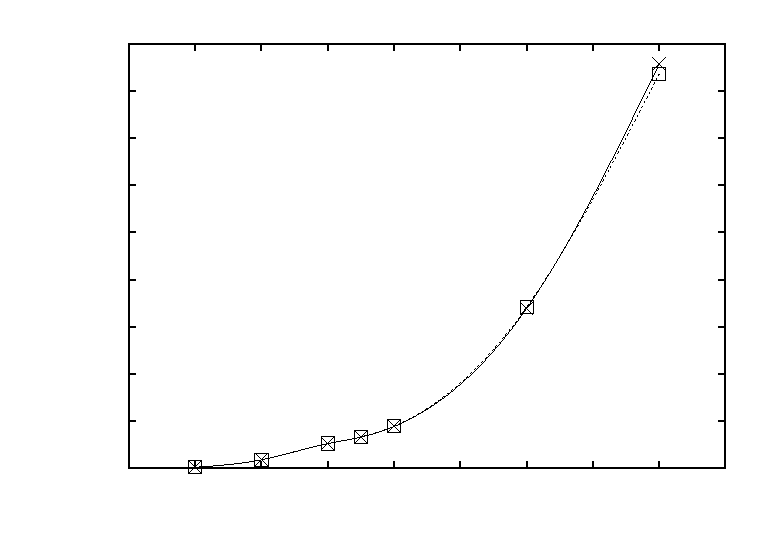
\includegraphics{plots/naive_at}}%
    \gplfronttext
  \end{picture}%
\endgroup

        \caption{Naïve Implementation Actual Times}
        \label{fig:naive_at}
    \end{center}
\end{figure}

\subsection{Discussion}

\section{MinHashing}\label{sec:minhashing}
MinHashing is a way of compressing the information stored in the characteristic matrix into space efficient signatures without loosing too much accuracy. MinHashing reduces the number of rows in the characteristic matrix. The number of columns stays the same.\\

Signatures are produced by first permuting the rows in the characteristic matrix. After the rows have been permuted we proceed by looking at the first column where we search until we find the first 1 where we read the index number. We do this for all columns. The signature is then the list of index numbers. This signature matrix is one row. To gain more accuracy we can permute the rows $k$ times and repeat the search for 1s. $k$ is the number of rows in the signiture matrix.

\subsection{Permutations and the simulating of these}
Since the permutation of such a large matrix is infeasible, we create a number of hash functions, $h_1, ..., h_k$, which should be less than the number of rows in the characteristic matrix. \\

Remarkably, the probability that the minhash function produces the same value for two sets is the same as the Jaccard similarity of the two sets (p. 82 in \cite{book:mmds}). Let \\

    $x = $ the rows in which the two sets both have a 1. \\
    $y = $ the rows in which one of the sets have a 1. \\
    $z = $ the rows in which none of the sets have a 1. \\

Then the probability of having found a row in $x$, for a random permutation, is

\begin{equation*}
    \frac{x}{x+y}
\end{equation*}

which is equals to the Jaccard similarity of the two sets.

\begin{equation*}
    \frac{|S_1 \cap S_2|}{|S_1 \cup S_2|} = \frac{x}{x+y}
\end{equation*}
    
We simulate $k$ random permutations by creating $k$ number of random hash functions \footnote{We are using universal hashing ($(ax + b) \bmod p$) as our hashing functions, where there will be some collisions in the hashes. Some row indexes will be hashed to the same, but as long as $k$ is large it is not important (p. 83-84 in \cite{book:mmds}).}. All row indices are then hashed with all these hash functions, to simulate a permutation. When this is done we proceed to making the signature matrix, which is a $k\times n$ matrix, that contains the minimum value of $h(x)$, where $x$ is an element in $S$. This is like finding the first 1 in each column. See figure ~\ref{fig:signature_matrix}\\

\begin{figure}[H]
    \begin{eqnarray*}
     & n \ \text{signatures} \\
     k \ \text{permutations} = & 
        \begin{cases}
        \overbrace{
        \begin{bmatrix}
            1 & 1 & 4 & 3 & 3 & 6 & 4\\
            3 & 3 & 1 & 5 & 3 & 2 & 1\\
            4 & 3 & 2 & 3 & 3 & 4 & 5\\
            0 & 1 & 4 & 2 & 2 & 6 & 1\\
        \end{bmatrix} 
        } 
        \end{cases}
    \end{eqnarray*}
    \caption{Signature matrix}
    \label{fig:signature_matrix}
\end{figure}

The above described method for calculating similarities are described in detail in our pseudo code in algorithm \ref{alg:minhashing}. This forms the basis for our implementation.

\begin{center}   
    \captionof{algorithm}[hypcap=false]{MinHashing algorithm}\label{alg:minhashing}
    \begin{algorithmic}
    \State $M\gets \text{characteristic matrix dictionary}$
    \State $a\gets \text{actors}$
    \State $m\gets \text{movies}$
    \State $k\gets \text{number of permutations}$\\
    \BState \emph{Declare signature matrix}:
    \State $SIG\gets \text{matrix with dimensions } a.length \times k$
    \ForAll{$i$ in $SIG$} 
        \State $i\gets \infty$
    \EndFor\\
    \BState \emph{Define hash functions}:
    \State $H\gets \text{empty list of universal hash functions, length }k$
    \State $p\gets \text{prime number larger than } k$
    \ForAll{$h_{\pi}$ in $H$} 
        \State $a\gets \text{random integer from } 1 \ldots p$
        \State $b\gets \text{random integer from } 0 \ldots p$
        \State $h_{\pi}\gets (a, b, p)$
    \EndFor\\
    \BState \emph{Populate signature matrix}:
    \ForAll{$(i,j)$ in $M$} 
        \For{$\pi$ in $0 \ldots k$}
            \State $v \gets h_{\pi}(j)$
            \If{$v<SIG[i,\pi]$}
                \State $SIG[i,\pi] = v$
            \EndIf
        \EndFor
    \EndFor\\
    \BState \emph{Calculate similarity}:
    \State $similarity \gets \text{empty dictionary}$ 
    \ForAll{pairs $a_i, a_j$ in $actors$}
        \State $c \gets 0$ number of collisions
        \For{$\pi$ in $0 \ldots k$}
            \If{$SIG[i,\pi] = SIG[j,\pi]$}
                \State $c += 1$
            \EndIf
        \EndFor
        \State $similarity[a_i,a_j] \gets \frac{c}{k}$ 
    \EndFor
    \end{algorithmic}
\end{center}

As in the naïve solution, we still have to compare all pairs of actors, but the number values needed to compared for each pair of actors is reduced from $m$ to $k$, resulting in a new running time $O(n^2 \cdot k)$ compared to previous $O(n^2 \cdot m)$, see figure ~\ref{fig:char_matrix} versus ~\ref{fig:signature_matrix}.

\subsection{Actual Running Times}
In figure ~\ref{fig:minhashing_at} the actual running times can be seen with different values for $k$. The running time for the naive solution is also plotted in this graph so one can see the difference in performance. \\


\begin{figure}[H]
    \begin{center}
        % GNUPLOT: LaTeX picture with Postscript
\begingroup
  \makeatletter
  \providecommand\color[2][]{%
    \GenericError{(gnuplot) \space\space\space\@spaces}{%
      Package color not loaded in conjunction with
      terminal option `colourtext'%
    }{See the gnuplot documentation for explanation.%
    }{Either use 'blacktext' in gnuplot or load the package
      color.sty in LaTeX.}%
    \renewcommand\color[2][]{}%
  }%
  \providecommand\includegraphics[2][]{%
    \GenericError{(gnuplot) \space\space\space\@spaces}{%
      Package graphicx or graphics not loaded%
    }{See the gnuplot documentation for explanation.%
    }{The gnuplot epslatex terminal needs graphicx.sty or graphics.sty.}%
    \renewcommand\includegraphics[2][]{}%
  }%
  \providecommand\rotatebox[2]{#2}%
  \@ifundefined{ifGPcolor}{%
    \newif\ifGPcolor
    \GPcolorfalse
  }{}%
  \@ifundefined{ifGPblacktext}{%
    \newif\ifGPblacktext
    \GPblacktexttrue
  }{}%
  % define a \g@addto@macro without @ in the name:
  \let\gplgaddtomacro\g@addto@macro
  % define empty templates for all commands taking text:
  \gdef\gplbacktext{}%
  \gdef\gplfronttext{}%
  \makeatother
  \ifGPblacktext
    % no textcolor at all
    \def\colorrgb#1{}%
    \def\colorgray#1{}%
  \else
    % gray or color?
    \ifGPcolor
      \def\colorrgb#1{\color[rgb]{#1}}%
      \def\colorgray#1{\color[gray]{#1}}%
      \expandafter\def\csname LTw\endcsname{\color{white}}%
      \expandafter\def\csname LTb\endcsname{\color{black}}%
      \expandafter\def\csname LTa\endcsname{\color{black}}%
      \expandafter\def\csname LT0\endcsname{\color[rgb]{1,0,0}}%
      \expandafter\def\csname LT1\endcsname{\color[rgb]{0,1,0}}%
      \expandafter\def\csname LT2\endcsname{\color[rgb]{0,0,1}}%
      \expandafter\def\csname LT3\endcsname{\color[rgb]{1,0,1}}%
      \expandafter\def\csname LT4\endcsname{\color[rgb]{0,1,1}}%
      \expandafter\def\csname LT5\endcsname{\color[rgb]{1,1,0}}%
      \expandafter\def\csname LT6\endcsname{\color[rgb]{0,0,0}}%
      \expandafter\def\csname LT7\endcsname{\color[rgb]{1,0.3,0}}%
      \expandafter\def\csname LT8\endcsname{\color[rgb]{0.5,0.5,0.5}}%
    \else
      % gray
      \def\colorrgb#1{\color{black}}%
      \def\colorgray#1{\color[gray]{#1}}%
      \expandafter\def\csname LTw\endcsname{\color{white}}%
      \expandafter\def\csname LTb\endcsname{\color{black}}%
      \expandafter\def\csname LTa\endcsname{\color{black}}%
      \expandafter\def\csname LT0\endcsname{\color{black}}%
      \expandafter\def\csname LT1\endcsname{\color{black}}%
      \expandafter\def\csname LT2\endcsname{\color{black}}%
      \expandafter\def\csname LT3\endcsname{\color{black}}%
      \expandafter\def\csname LT4\endcsname{\color{black}}%
      \expandafter\def\csname LT5\endcsname{\color{black}}%
      \expandafter\def\csname LT6\endcsname{\color{black}}%
      \expandafter\def\csname LT7\endcsname{\color{black}}%
      \expandafter\def\csname LT8\endcsname{\color{black}}%
    \fi
  \fi
  \setlength{\unitlength}{0.0500bp}%
  \begin{picture}(7200.00,5040.00)%
    \gplgaddtomacro\gplbacktext{%
      \csname LTb\endcsname%
      \put(946,704){\makebox(0,0)[r]{\strut{} 0}}%
      \put(946,1286){\makebox(0,0)[r]{\strut{} 50}}%
      \put(946,1867){\makebox(0,0)[r]{\strut{} 100}}%
      \put(946,2449){\makebox(0,0)[r]{\strut{} 150}}%
      \put(946,3030){\makebox(0,0)[r]{\strut{} 200}}%
      \put(946,3612){\makebox(0,0)[r]{\strut{} 250}}%
      \put(946,4193){\makebox(0,0)[r]{\strut{} 300}}%
      \put(946,4775){\makebox(0,0)[r]{\strut{} 350}}%
      \put(1078,484){\makebox(0,0){\strut{} 0}}%
      \put(1714,484){\makebox(0,0){\strut{} 1}}%
      \put(2350,484){\makebox(0,0){\strut{} 2}}%
      \put(2986,484){\makebox(0,0){\strut{} 3}}%
      \put(3622,484){\makebox(0,0){\strut{} 4}}%
      \put(4259,484){\makebox(0,0){\strut{} 5}}%
      \put(4895,484){\makebox(0,0){\strut{} 6}}%
      \put(5531,484){\makebox(0,0){\strut{} 7}}%
      \put(6167,484){\makebox(0,0){\strut{} 8}}%
      \put(6803,484){\makebox(0,0){\strut{} 9}}%
      \put(176,2739){\rotatebox{-270}{\makebox(0,0){\strut{}Time (s)}}}%
      \put(3940,154){\makebox(0,0){\strut{}Input data size (x100 movies | x1000 roles)}}%
    }%
    \gplgaddtomacro\gplfronttext{%
      \csname LTb\endcsname%
      \put(2704,4083){\makebox(0,0)[r]{\strut{}k=5}}%
      \csname LTb\endcsname%
      \put(2704,3863){\makebox(0,0)[r]{\strut{}k=10}}%
      \csname LTb\endcsname%
      \put(2704,3643){\makebox(0,0)[r]{\strut{}k=20}}%
      \csname LTb\endcsname%
      \put(2704,3423){\makebox(0,0)[r]{\strut{}k=40}}%
    }%
    \gplbacktext
    \put(0,0){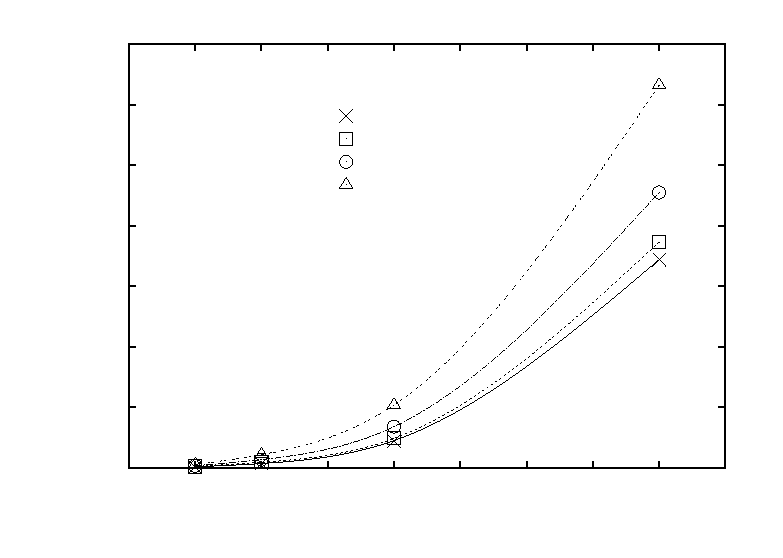
\includegraphics{plots/minhashing_at}}%
    \gplfronttext
  \end{picture}%
\endgroup

        \caption{MinHashing Actual Times}
        \label{fig:minhashing_at}
    \end{center}
\end{figure}

\subsection{Discussion}

\section{Locality Sensitive Hashing (LSH)}
Locality sensitive hashing is a way of coping with an even larger amount of data than MinHashing can. So if the number of pairs is too large, LSH is an option to use. We take the signatures produced by min hashing and chop them up into shorter vectors by dividing the total number of rows into $b$ bands of $r$ rows. We then save the vectors into a hashtable (here referred to as a bucket), in such a way that if two vectors are similar, they are put in the bucket. If a bucket has two or more vectors in it, then the signatures containing these vectors become candidate pairs. When comparing for similarity, we then only compare candidate pairs. This leaves us with a significant fraction of the original set of pairs to check. \\

In figure \ref{fig:lsh_buckets} the signature matrix from earlier has been dissected into two bands. These bands have, in this example, the same number of buckets as there are signatures. The buckets containing 2 or more signatures have been marked in green. If a signature is in one or more buckets it is a candidate signature to be checked for similarity, whereas if a signature is only in red buckets, which have only one or zero signatures, it is discarded as a candidate signature. \\

So the candidate signatures are $S_0, S_1, S_3, S_4, S_6$, and the discarded signatures are $S_2, S_5$.

\begin{figure}[H]
    \begin{center}
        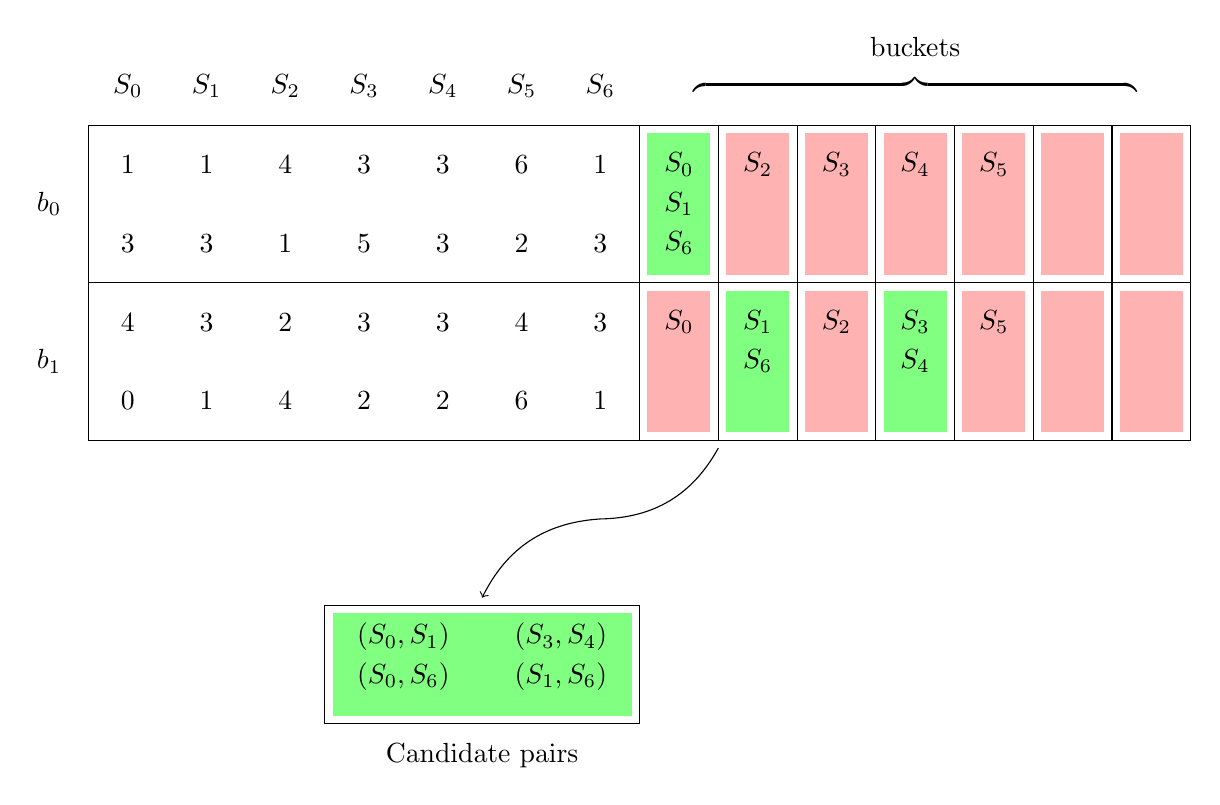
\begin{tikzpicture}
            \draw rectangle (14,4);
            \draw rectangle (7,2);
            \draw (0,2) rectangle (7,2);
            \draw (7,0) rectangle (8,4);

            \foreach \x in {0,...,6} \draw (\x+7, 0) rectangle (\x+7+1, 2);
            \foreach \x in {0,...,6} \draw (\x+7, 2) rectangle (\x+7+1, 4);
            \foreach \x in {0,...,6} \draw (\x+.5, 4.5) node {$S_\x$};

            \draw (-.5,3) node {$b_0$};
            \draw (-.5,1) node {$b_1$};

            % The overbrace
            \draw (10.5, 4.5) node {$\overbrace{\qquad\qquad\qquad\qquad\qquad\qquad\qquad\qquad}$};
            \draw (10.5,5.0) node {buckets};

            % Signature matrix (left part)
            \draw (0.5,3.5) node {1};
            \draw (0.5,2.5) node {3};
            \draw (0.5,1.5) node {4};
            \draw (0.5,0.5) node {0};

            \draw (1.5,3.5) node {1};
            \draw (1.5,2.5) node {3};
            \draw (1.5,1.5) node {3};
            \draw (1.5,0.5) node {1};

            \draw (2.5,3.5) node {4};
            \draw (2.5,2.5) node {1};
            \draw (2.5,1.5) node {2};
            \draw (2.5,0.5) node {4};

            \draw (3.5,3.5) node {3};
            \draw (3.5,2.5) node {5};
            \draw (3.5,1.5) node {3};
            \draw (3.5,0.5) node {2};

            \draw (4.5,3.5) node {3};
            \draw (4.5,2.5) node {3};
            \draw (4.5,1.5) node {3};
            \draw (4.5,0.5) node {2};

            \draw (5.5,3.5) node {6};
            \draw (5.5,2.5) node {2};
            \draw (5.5,1.5) node {4};
            \draw (5.5,0.5) node {6};

            \draw (6.5,3.5) node {1};
            \draw (6.5,2.5) node {3};
            \draw (6.5,1.5) node {3};
            \draw (6.5,0.5) node {1};

            % Fill all with red (in right part)
            \foreach \x in {0,...,6} \path[fill=red!30] (7.1+\x,0.1) rectangle (7.9+\x,1.9);
            \foreach \x in {0,...,6} \path[fill=red!30] (7.1+\x,2.1) rectangle (7.9+\x,3.9);

            % Fill the right ones with green
            \path[fill=green!50] (7.1,2.1) rectangle (7.9,3.9);
            \path[fill=green!50] (8.1,0.1) rectangle (8.9,1.9);
            \path[fill=green!50] (10.1,0.1) rectangle (10.9,1.9);

            % Names
            \draw (7.5,3.5) node {$S_0$};
            \draw (7.5,3.0) node {$S_1$};
            \draw (7.5,2.5) node {$S_6$};
            \draw (8.5,3.5) node {$S_2$};
            \draw (9.5,3.5) node {$S_3$};
            \draw (10.5,3.5) node {$S_4$};
            \draw (11.5,3.5) node {$S_5$};

            \draw (7.5,1.5) node {$S_0$};
            \draw (8.5,1.5) node {$S_1$};
            \draw (8.5,1.0) node {$S_6$};
            \draw (9.5,1.5) node {$S_2$};
            \draw (10.5,1.5) node {$S_3$};
            \draw (10.5,1.0) node {$S_4$};
            \draw (11.5,1.5) node {$S_5$};


            % Arrows
            \path[-] (8,-.1) edge [bend left] (6.5,-1);
            \path[->] (6.5,-1) edge [bend right] (5,-2);

            % Candidate squares
            \path[fill=green!50] (3.1, -3.5) rectangle (6.9, -2.2);
            \draw (3,-3.6) rectangle (7,-2.1);

            % Candidate signatures
            \draw (4,-2.5) node {$(S_0, S_1)$};
            \draw (4,-3.0) node {$(S_0, S_6)$};
            \draw (6,-3.0) node {$(S_1, S_6)$};
            \draw (6,-2.5) node {$(S_3, S_4)$};

            \draw (5,-4.0) node {Candidate pairs};
            

        \end{tikzpicture}
    \caption{LSH buckets and bands}
    \label{fig:lsh_buckets}
    \end{center}
\end{figure}

We concatenate the integers of the r rows in to a single string and then uses this as a key for a dictionary, which is essential a hash table. This gives us our desired result of identical bands of signatures hashes to the same value with high probability. We create a hash table for each band, and then for each key, we create a list\footnote{a bucket} and add the signature id to it. Every time we find key that already present in the  hash table we add the signature id to the existing bucket. The follow pseudo code in algorithm \ref{alg:lsh} describes this. 

\begin{center}   
    \captionof{algorithm}{Locallity Similarity Hashing algorithm}\label{alg:lsh}
    \begin{algorithmic}
    
    \BState \textbf{Calculate signature matrix as in algorithm \ref{alg:minhashing}}\\

    \State $SIG\gets \text{signature matrix}$
    \State $S\gets \text{number of signatures}$
    \State $bucket\_list\gets \text{empty list}$
    \State $B\gets \text{number of bands}$\\

    \BState \emph{Fill the buckets}
    \For{$b_i$ in $i = 0 \ldots B-1$}
        \State $h_i \gets \text{empty dictionary}$
        \State $bucket\_list.append(h_i)$
        \For{$SIG_j[b_i]$ in $j = 0 \ldots S-1$}
            \State $key \gets SIG_j[b_i]$
            \If{$key$ in $h_i$}
                \State $bucket \gets h_i[key]$
            \Else
                \State $bucket \gets \text{empty list}$
            \EndIf
            \State $bucket.append(j)$
        \EndFor
    \EndFor\\

    \State $candidate\_pairs \gets \text{empty set}$
    \ForAll{$h_i$ in $bucket\_list$}
        \ForAll{$key$ in $h_i$}
            \State $bucket \gets h_i[key]$
            \If{$bucket.length > 1$}
                \For{$pair$ in $bucket$}
                    \State $candidate\_pairs.add(pair)$ 
                \EndFor
            \EndIf
        \EndFor        
    \EndFor\\

    \BState \textbf{Calculate similarities from signature matrix as in algorithm \ref{alg:minhashing}, for the candidate pairs.}

    \end{algorithmic}
\end{center}

\subsection{Analysis}
In the worst case example, we would get all pairs to be candidate pairs, and the time complexity would be $O(n^2)$ in LSH. But to get to LSH, we would have to do MinHashing first, to get the signature matrix\todo{incorrect}, and MinHashing has a time complexity of $O(n^2k)$. Hopefully, we can discard many signatures, so we only have a fraction as candidate pairs. By looking at the tuning parameters $b$ and $r$, we can calculate the probability $s$ that two signatures will become a candidate pair. \\

By tuning $r$ and $b$, we can state how similar we will allow pairs to be. In the figure \ref{fig:scurve} is plotted three curves of the formula \ref{eq:s} with different $r$, and $b$ values. These are plots of the probability that two signatures will become candidate pairs. At the point on the curves where the value on the y-axis is 0.5, is the \emph{threshold} point\footnote{This is about the point where the curve is the steepest}. When we have a pair with a similarity equivalent to this point, we know that there is a $50\%$ probability that is will become a candidate pair. \\

\begin{equation}
    \text {Probability} = 1 - (1 - s^r)^b 
    \label{eq:s}
\end{equation}\\

If we bring this curve further to the right - using our tuning parameters $r$, and $b$ - a pair would need to have a higher similarity to have a probability of becoming a candidate pair. To approximately find the threshold point, equation \ref{eq:s-estimate} can be used.  \\


\begin{figure}[H]
    \begin{center}
        % GNUPLOT: LaTeX picture with Postscript
\begingroup
  \makeatletter
  \providecommand\color[2][]{%
    \GenericError{(gnuplot) \space\space\space\@spaces}{%
      Package color not loaded in conjunction with
      terminal option `colourtext'%
    }{See the gnuplot documentation for explanation.%
    }{Either use 'blacktext' in gnuplot or load the package
      color.sty in LaTeX.}%
    \renewcommand\color[2][]{}%
  }%
  \providecommand\includegraphics[2][]{%
    \GenericError{(gnuplot) \space\space\space\@spaces}{%
      Package graphicx or graphics not loaded%
    }{See the gnuplot documentation for explanation.%
    }{The gnuplot epslatex terminal needs graphicx.sty or graphics.sty.}%
    \renewcommand\includegraphics[2][]{}%
  }%
  \providecommand\rotatebox[2]{#2}%
  \@ifundefined{ifGPcolor}{%
    \newif\ifGPcolor
    \GPcolorfalse
  }{}%
  \@ifundefined{ifGPblacktext}{%
    \newif\ifGPblacktext
    \GPblacktexttrue
  }{}%
  % define a \g@addto@macro without @ in the name:
  \let\gplgaddtomacro\g@addto@macro
  % define empty templates for all commands taking text:
  \gdef\gplbacktext{}%
  \gdef\gplfronttext{}%
  \makeatother
  \ifGPblacktext
    % no textcolor at all
    \def\colorrgb#1{}%
    \def\colorgray#1{}%
  \else
    % gray or color?
    \ifGPcolor
      \def\colorrgb#1{\color[rgb]{#1}}%
      \def\colorgray#1{\color[gray]{#1}}%
      \expandafter\def\csname LTw\endcsname{\color{white}}%
      \expandafter\def\csname LTb\endcsname{\color{black}}%
      \expandafter\def\csname LTa\endcsname{\color{black}}%
      \expandafter\def\csname LT0\endcsname{\color[rgb]{1,0,0}}%
      \expandafter\def\csname LT1\endcsname{\color[rgb]{0,1,0}}%
      \expandafter\def\csname LT2\endcsname{\color[rgb]{0,0,1}}%
      \expandafter\def\csname LT3\endcsname{\color[rgb]{1,0,1}}%
      \expandafter\def\csname LT4\endcsname{\color[rgb]{0,1,1}}%
      \expandafter\def\csname LT5\endcsname{\color[rgb]{1,1,0}}%
      \expandafter\def\csname LT6\endcsname{\color[rgb]{0,0,0}}%
      \expandafter\def\csname LT7\endcsname{\color[rgb]{1,0.3,0}}%
      \expandafter\def\csname LT8\endcsname{\color[rgb]{0.5,0.5,0.5}}%
    \else
      % gray
      \def\colorrgb#1{\color{black}}%
      \def\colorgray#1{\color[gray]{#1}}%
      \expandafter\def\csname LTw\endcsname{\color{white}}%
      \expandafter\def\csname LTb\endcsname{\color{black}}%
      \expandafter\def\csname LTa\endcsname{\color{black}}%
      \expandafter\def\csname LT0\endcsname{\color{black}}%
      \expandafter\def\csname LT1\endcsname{\color{black}}%
      \expandafter\def\csname LT2\endcsname{\color{black}}%
      \expandafter\def\csname LT3\endcsname{\color{black}}%
      \expandafter\def\csname LT4\endcsname{\color{black}}%
      \expandafter\def\csname LT5\endcsname{\color{black}}%
      \expandafter\def\csname LT6\endcsname{\color{black}}%
      \expandafter\def\csname LT7\endcsname{\color{black}}%
      \expandafter\def\csname LT8\endcsname{\color{black}}%
    \fi
  \fi
  \setlength{\unitlength}{0.0500bp}%
  \begin{picture}(5400.00,3780.00)%
    \gplgaddtomacro\gplbacktext{%
      \csname LTb\endcsname%
      \put(946,704){\makebox(0,0)[r]{\strut{} 0}}%
      \put(946,1266){\makebox(0,0)[r]{\strut{} 0.2}}%
      \put(946,1828){\makebox(0,0)[r]{\strut{} 0.4}}%
      \put(946,2391){\makebox(0,0)[r]{\strut{} 0.6}}%
      \put(946,2953){\makebox(0,0)[r]{\strut{} 0.8}}%
      \put(946,3515){\makebox(0,0)[r]{\strut{} 1}}%
      \put(1078,484){\makebox(0,0){\strut{} 0}}%
      \put(1863,484){\makebox(0,0){\strut{} 0.2}}%
      \put(2648,484){\makebox(0,0){\strut{} 0.4}}%
      \put(3433,484){\makebox(0,0){\strut{} 0.6}}%
      \put(4218,484){\makebox(0,0){\strut{} 0.8}}%
      \put(5003,484){\makebox(0,0){\strut{} 1}}%
      \put(176,2109){\rotatebox{-270}{\makebox(0,0){\strut{}Probability of becoming a candidate pair}}}%
      \put(3040,154){\makebox(0,0){\strut{}Jaccard similarity}}%
    }%
    \gplgaddtomacro\gplfronttext{%
      \csname LTb\endcsname%
      \put(2515,3124){\makebox(0,0)[r]{\strut{}r=25, b=40}}%
      \csname LTb\endcsname%
      \put(2515,2904){\makebox(0,0)[r]{\strut{}r=20, b=50}}%
      \csname LTb\endcsname%
      \put(2515,2684){\makebox(0,0)[r]{\strut{}r=10, b=100}}%
    }%
    \gplbacktext
    \put(0,0){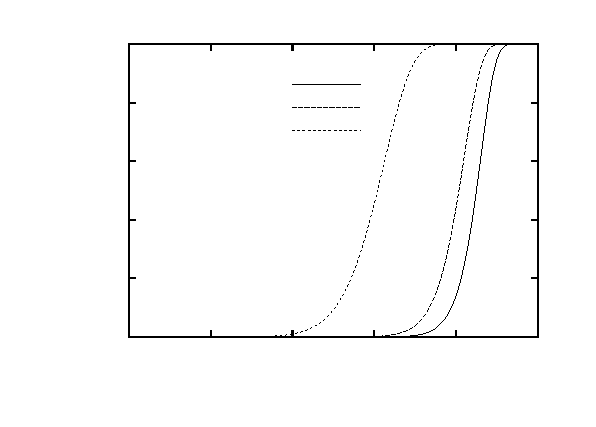
\includegraphics{plots/scurve}}%
    \gplfronttext
  \end{picture}%
\endgroup

        \caption{S-curve - $f(s) = 1 - (1 - s^r)^b$}
        \label{fig:scurve}
    \end{center}
\end{figure}

The three S-curves in figure \ref{fig:scurve} have the following threshold values, $[0.63, 0.82, 0.86]$, which means that on the curve with threshold $0.63$\footnote{with $b=10$ and $r=100$}, if we have a pair with similarity $0.5$, there is $63\%$ chance of it becoming a candidate pair. \\

For every band, a pair has about $1 - (\left(1-s^r \right)$ chance of being regarded as similar, which is not necessarily much. But there are $b$ bands in which this is applicable, which raises the chance of the pair becoming a candidate pair. \\

There is always a probability of a similar pair not becoming a candidate pair and vice versa. These are false negatives and false positives. False positives will be chosen as candidate pairs without being similar, and false negatives will not be chosen as candidates even though they are similar. The S-curve can be tuned to match a high probability for either false positives or false negatives, depending on what is important to the problem. \todo{Hvad er vigtigst i dette project?}\\


\begin{equation}
    s = (1/b)^{1/r}
    \label{eq:s-estimate}
\end{equation}


\subsection{Actual Running Time}
The actual running times of LSH can be seen in figure \ref{fig:lsh_at} together with the naive running time, and one of the running times for MinHashing. This way one can see the change in performance.

\todo{Skal vi lave comparison af correctness?}

\begin{figure}[H]
    \begin{center}
        % GNUPLOT: LaTeX picture with Postscript
\begingroup
  \makeatletter
  \providecommand\color[2][]{%
    \GenericError{(gnuplot) \space\space\space\@spaces}{%
      Package color not loaded in conjunction with
      terminal option `colourtext'%
    }{See the gnuplot documentation for explanation.%
    }{Either use 'blacktext' in gnuplot or load the package
      color.sty in LaTeX.}%
    \renewcommand\color[2][]{}%
  }%
  \providecommand\includegraphics[2][]{%
    \GenericError{(gnuplot) \space\space\space\@spaces}{%
      Package graphicx or graphics not loaded%
    }{See the gnuplot documentation for explanation.%
    }{The gnuplot epslatex terminal needs graphicx.sty or graphics.sty.}%
    \renewcommand\includegraphics[2][]{}%
  }%
  \providecommand\rotatebox[2]{#2}%
  \@ifundefined{ifGPcolor}{%
    \newif\ifGPcolor
    \GPcolorfalse
  }{}%
  \@ifundefined{ifGPblacktext}{%
    \newif\ifGPblacktext
    \GPblacktexttrue
  }{}%
  % define a \g@addto@macro without @ in the name:
  \let\gplgaddtomacro\g@addto@macro
  % define empty templates for all commands taking text:
  \gdef\gplbacktext{}%
  \gdef\gplfronttext{}%
  \makeatother
  \ifGPblacktext
    % no textcolor at all
    \def\colorrgb#1{}%
    \def\colorgray#1{}%
  \else
    % gray or color?
    \ifGPcolor
      \def\colorrgb#1{\color[rgb]{#1}}%
      \def\colorgray#1{\color[gray]{#1}}%
      \expandafter\def\csname LTw\endcsname{\color{white}}%
      \expandafter\def\csname LTb\endcsname{\color{black}}%
      \expandafter\def\csname LTa\endcsname{\color{black}}%
      \expandafter\def\csname LT0\endcsname{\color[rgb]{1,0,0}}%
      \expandafter\def\csname LT1\endcsname{\color[rgb]{0,1,0}}%
      \expandafter\def\csname LT2\endcsname{\color[rgb]{0,0,1}}%
      \expandafter\def\csname LT3\endcsname{\color[rgb]{1,0,1}}%
      \expandafter\def\csname LT4\endcsname{\color[rgb]{0,1,1}}%
      \expandafter\def\csname LT5\endcsname{\color[rgb]{1,1,0}}%
      \expandafter\def\csname LT6\endcsname{\color[rgb]{0,0,0}}%
      \expandafter\def\csname LT7\endcsname{\color[rgb]{1,0.3,0}}%
      \expandafter\def\csname LT8\endcsname{\color[rgb]{0.5,0.5,0.5}}%
    \else
      % gray
      \def\colorrgb#1{\color{black}}%
      \def\colorgray#1{\color[gray]{#1}}%
      \expandafter\def\csname LTw\endcsname{\color{white}}%
      \expandafter\def\csname LTb\endcsname{\color{black}}%
      \expandafter\def\csname LTa\endcsname{\color{black}}%
      \expandafter\def\csname LT0\endcsname{\color{black}}%
      \expandafter\def\csname LT1\endcsname{\color{black}}%
      \expandafter\def\csname LT2\endcsname{\color{black}}%
      \expandafter\def\csname LT3\endcsname{\color{black}}%
      \expandafter\def\csname LT4\endcsname{\color{black}}%
      \expandafter\def\csname LT5\endcsname{\color{black}}%
      \expandafter\def\csname LT6\endcsname{\color{black}}%
      \expandafter\def\csname LT7\endcsname{\color{black}}%
      \expandafter\def\csname LT8\endcsname{\color{black}}%
    \fi
  \fi
  \setlength{\unitlength}{0.0500bp}%
  \begin{picture}(7200.00,5040.00)%
    \gplgaddtomacro\gplbacktext{%
      \csname LTb\endcsname%
      \put(814,704){\makebox(0,0)[r]{\strut{} 0}}%
      \put(814,1518){\makebox(0,0)[r]{\strut{} 10}}%
      \put(814,2332){\makebox(0,0)[r]{\strut{} 20}}%
      \put(814,3147){\makebox(0,0)[r]{\strut{} 30}}%
      \put(814,3961){\makebox(0,0)[r]{\strut{} 40}}%
      \put(814,4775){\makebox(0,0)[r]{\strut{} 50}}%
      \put(946,484){\makebox(0,0){\strut{} 0}}%
      \put(1597,484){\makebox(0,0){\strut{} 1}}%
      \put(2248,484){\makebox(0,0){\strut{} 2}}%
      \put(2898,484){\makebox(0,0){\strut{} 3}}%
      \put(3549,484){\makebox(0,0){\strut{} 4}}%
      \put(4200,484){\makebox(0,0){\strut{} 5}}%
      \put(4851,484){\makebox(0,0){\strut{} 6}}%
      \put(5501,484){\makebox(0,0){\strut{} 7}}%
      \put(6152,484){\makebox(0,0){\strut{} 8}}%
      \put(6803,484){\makebox(0,0){\strut{} 9}}%
      \put(176,2739){\rotatebox{-270}{\makebox(0,0){\strut{}Time (s)}}}%
      \put(3874,154){\makebox(0,0){\strut{}x100 movies | x1000 actors}}%
    }%
    \gplgaddtomacro\gplfronttext{%
      \csname LTb\endcsname%
      \put(5885,4258){\makebox(0,0)[r]{\strut{}b=10, r=2}}%
      \csname LTb\endcsname%
      \put(5885,4038){\makebox(0,0)[r]{\strut{}b=10, r=5}}%
      \csname LTb\endcsname%
      \put(5885,3818){\makebox(0,0)[r]{\strut{}b=25, r=2}}%
      \csname LTb\endcsname%
      \put(5885,3598){\makebox(0,0)[r]{\strut{}MinHash k=10}}%
      \csname LTb\endcsname%
      \put(5885,3378){\makebox(0,0)[r]{\strut{}naive}}%
    }%
    \gplbacktext
    \put(0,0){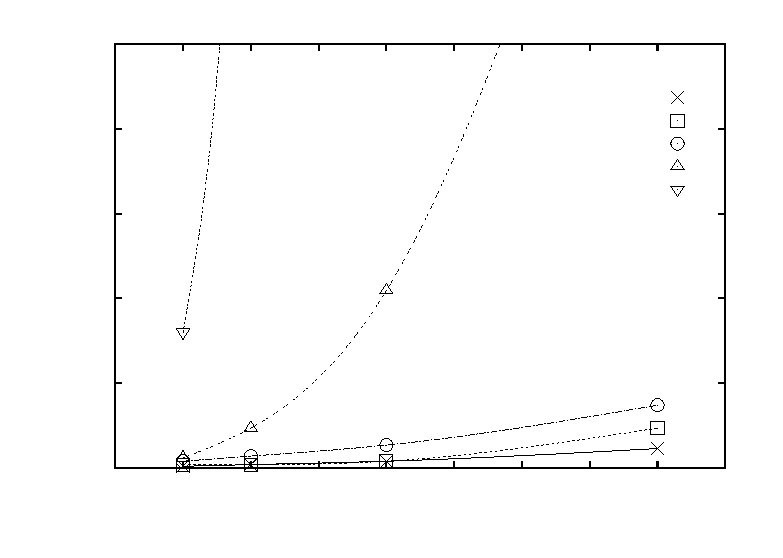
\includegraphics{plots/lsh_at}}%
    \gplfronttext
  \end{picture}%
\endgroup

        \caption{LSH Actual Times}
        \label{fig:lsh_at}
    \end{center}
\end{figure}

\subsection{Discussion}

\section{B-bit}
B-bit MinHashing is a way to estimate set similarity in a more storage efficient way than with MinHashing alone. It is a modification for MinHashing. The time complexity remains $O(n^2k)$, but out of every signature, only the last few bits are saved. This simulates a low level hashing function, where dissimilar documents could be hashed to the same b-bit value. \\

In our project we have found difficulties getting \emph{Python} to store a bit value using less space than an integer below $2^{30}-1 = 1,073,741,823$, or just about 1 billion\footnote{All our objects (integers) would in Python have a size of 8 bytes, not counting the overhead.}. This means we can not gain much in space complexity using python, since our dataset is only in the scale of millions of distinct object. We will have to cluster the binary values from every signature together in a single integer, and do bitwise operations on that. This is proposed in \cite{article:bbit} section 5.1. Though we have not been able to implement this, and therefore our b-bit is nonfunctional. \\

If we are able to store one object using only 1 bit, we only use as many bits, as we have objects. If we have $n$ objects, and they all originally have a minimum size of $s = 8 \cdot 8 = 64$ bits, we would at most use $1/s = 1/64$ of the original space. Notice that the time complexity is still the same. \\

Say we had some hardware that could do boolean comparisons faster than integer comparisons, then a b-bit implementation could utilize this functionality. But that is out of scope of this course. \\


\subsection{The Variance-Space tradeoff}
The variance in our project is a measure of how accurate our results are. We can store about 64 times as many samples when converting to 1 bit, but we lose some accuracy. This is the tradeoff, and can be precisely quantified by the storage factor, which calculates the ratio of the  storage. See equation \ref{eq:storagefactor}.

\begin{equation}
    \text {Storage factor} = B(b;R,r_1,r_2)
    \label{eq:storagefactor}
\end{equation}

Where:\\
$b = $ the number of bits used to store an object. \\
$R = $ the resemblance between two objects \\
$r_1 = $ percentage of total elements in $S_1$ \\
$r_2 = $ percentage of total elements in $S_2$ \\

In \cite{article:bbit} section 2.3, it is deduced that the improvements from using 64 bits to using 1 bit will at least be 21.3-fold. Let us state that $b_1 = 64$ and $b_2 = 1$, then the improvement ratio between the two will be

\begin{equation}
    \frac{B(64;R,r_1,r_2)}{B(1;R,r_1,r_2} \Rightarrow \frac{64 R}{R + 1 - r_1}
    \label{eq:improvementratio}
\end{equation}

In the best case, $R = r_1 = r_2 = 1$, and the improvement ratio will be $\frac{64}{1}$. In the worst case, the resemblance, $R=.5$, and $r_1, r_2 \rightarrow 0$ the ratio will be $\frac{64}{3} \sim 21.3$. See figure \ref{fig:bbit} to see a graph from \cite{article:bbit} which shows the storage improvements with different parameters. \\


\begin{figure}[H]
    \begin{center}
        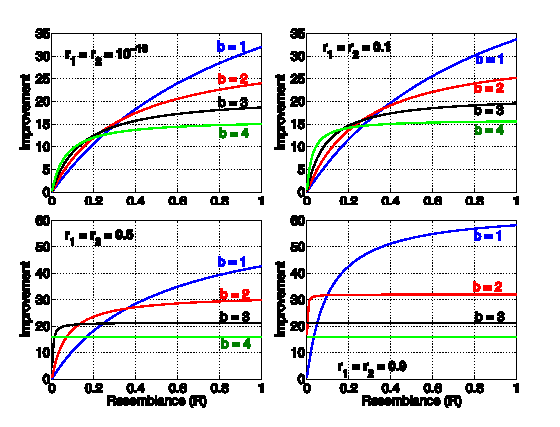
\includegraphics{plots/bbit/bbit.eps}
        \caption{B-bit storage improvement}
        \label{fig:bbit}
    \end{center}
\end{figure}


\subsection{Running Time}
Our implementation of the b-bit algorithm does not succesfully run on the imdb dataset, only on our dummy data. Part of the reasom for this is that we have not been able to implement a data type with a small enough overhead. So instead of our data actually taking up less space, it takes up the same space, and furthermore additional processing is done to it. See figure \ref{fig:bbit_at} for the actual running times.\\

\begin{figure}[H]
    \begin{center}
        %\input{plots/bbit_at.tex}
        \caption{B-bit actual running time}
        \label{fig:bbit_at}
    \end{center}
\end{figure}

\subsection{LSH versus b-Bit}
These two algorithms are both modifications to MinHashing. How do they compare to each other? Performance. What are their strengths?

\subsection{Discussion}

\section{Future Work}
Odd Sketch is good when you want to improve precision when the Jaccard similarity index is close to 1. It can provide a short list and ranking over the most similar items. \\



\subsection{Discussion}

\section{Conclusion}
\newpage
\bibliography{bibliography}
\begin{appendices}
\section{Code}
\lstinputlisting[language=Python]{../temp.py}
\end{appendices}
\end{document}

